\documentclass[14pt,a4]{extreport}
\usepackage{multirow,comment,amsmath,hyperref,array,longtable,amssymb,comment, lastpage,enumitem,framed,graphicx,adjustbox,multicol,xcolor}
\usepackage[a4paper, left=1.6cm, right=1.6cm, top=2.5cm, bottom=2.8cm]{geometry}

\graphicspath{ {./images/} }
\DeclareGraphicsExtensions{.pdf,.jpeg,.png}
%\usepackage{fontspec}
%\setmainfont{Arial}

\begin{document}
\begin{centering}
\vspace{1cm}
\Large{Department of Computer Science \& Engineering}\\ 
{\bf \LARGE Indian Institute of Information Technology Senapati}\\
\vspace{6cm}

%\vspace{2.5cm}
{\huge Application of dynamic programming and graph algorithms}\\
{(Course Code: CS 200)}\\
\vspace{4cm}
{\textsc{\Large Shivam Sharma} \\ 18010121\par}
\vspace{4cm}
Supervised by\\
\textsc{Dr. Kabita Thaoroijam} \par

\vfill
24 June 2020
\end{centering}


\begin{abstract}
Shortest path algorithms have many applications.Mapping software like Google or Apple maps makes use of shortest path algorithms.  They are also important for road network, operations, and logistics research.  Shortest path algorithms are also very important for computer networks, like the Internet.Shortest path algorithms have wide applications and so wide are no of algorithms to find shortest path.We always uses the google maps etc. to find shortest path while going from one place to another.This project will analyse how the maps actually finds the path using shortest path algorithms.In this we will analyse the time taken by different algorithms in finding the shortest path from source node to destination node.But the most important factor among all such algorithms are time and space complexity of  the  algorithms.We  always  want  to  use  system  which  gives  us  faster  results.
\end{abstract}



%\newpage
\chapter{Introduction}

The project introduces with the analysis of different pathfinding algorithms like DFS,BFS,Dijsktra and A* algorithm.
While analysing all the algorithms ,the project will compare how much time the given possible paths.
We always uses the google maps etc. to find shortest path while going from one place to another.This project will analyse how the maps actually finds the path using shortest path algorithms.In this we will analyse the time taken by different algorithms in finding the shortest path from source node to destination node.Shortest path algorithms have many applications.Mapping software like Google or Apple maps makes use of shortest path algorithms. They are also important for road network, operations, and logistics research. Shortest path algorithms are also very important for computer networks, like the Internet.Shortest path algorithms have wide applications and so wide are no of algorithms to find shortest path.But the most important factor among all such algorithms are time and space complexity of the algorithms.We always want to use system which gives us faster results.In this project , we will analyse the Shortest path algorithms such as Dijkstra's algorithm and Astar search Algorithm etc. for time taken by the algorithms to find the shortest path . This Project will also compares the shortest path algorithms over large dataset of nodes and edges for time taken by the algorithms. 
\section {Problem statement}

Task is to analyse various shortest path algorithms which includes Dijkstra's algorithm ,A star search algorithm etc. for their time complexity over large dataset.This project also compares between those algorithms over large graph dataset of road network which comprises 5 lac+ nodes and 20 lac+ edges.

\section {Motivation behind selection of the project}
Graph algorithms are used extensively in many daily life problems among which most important problem is to find shortest path between two points.That's why I wanted to study very deeply about graph algorithms especially pathfinding algorithms.Also I was fascinated by pathfinding algorithms, and I wanted to visualize them in action. Project was also based on dynamic programming which is most efficient algorithm.Dynamic programming stores the computed result and always uses the precomputed result whenever needed to optimise the time complexity.All the points mentioned above motivated me alot to choose this project.

\section{Roadmap}

Task is to find the shortest path between two cities of the given dataset.To complete the task this project implements Dijkstra's Algorithm and Astar algorithm for shortest path in C++ language.
Both the algorihtms will work over large dataset of road network of california city.The dataset comprises 
almost 5 lac+ nodes and 20 lac+ edges.

And another task is to compare the time taken by both the algorithms to find the shortest path .To do so ,a graph is also plotted using gnuplot between time taken by both algrithms and no of nodes used by using linux shell programs.

\section{Your contribution}
I have implemented Astar Algorithm and Dijktra's shortest path algorithm for finding the shortest path between two nodes (Two cities) of the graph.The Programs read the dataset of nodes and edges and form the corresponding graph data structure from the given data .The programs also expect the user to provide the destination node as command line input , the program then displays the time taken by the algorithm to find the shortest path and length of the shortest path.I have also written a shell script to analyse both the algorithms over large dataset for time taken and compare both the algorithms in terms of time taken by both the algorithms.
\section{System/Software used}
Following System/Software has been used in development of this project :\\
1.This Project is developed under the linux environment.\\
\textbf{2.Gnuplot} for plotting graph between the time taken by an algorithm and no. of nodes used.\\
3.Linux Shell environment for running shell files
4.GNU/G++ Compiler for Compiling C++ files.

\section{Implementation plan}
In this project Dijkstra's Algorithm and Astar algorithm for shortest path is implemented in C++.
Both the algorithms are implemented in C++ because C++ is a powerful general-purpose programming language.C++ supports different ways of programming like procedural, object-oriented, functional, and so on.C++ offers very important feature which is concept of the Object Oriented Programming.This makes C++ powerful as well as flexible.More importantly C++ offers wide support of STL.The C++ STL (Standard Template Library) is a powerful set of C++ template classes to provide general-purpose classes and functions with templates that implement many popular and commonly used algorithms and data structures like vectors, lists, queues, and stacks.
Graph Data structure is used in implementing both the algorithms.
Both the algorihtms will work over large dataset of road network of california city.The dataset comprises 
almost 5 lac+ nodes and 20 lac+ edges.A shell program will also monitor the time taken by both algorithm to find shortest path between two nodes(cities) of the graph (Road network) . A graph is also plotted using gnuplot between time taken by both algrithms and no of nodes used.Gnuplot is used to plot graph between the time taken by an algorithm and no. of nodes used.
Dynamic Programming is also used in this project to efficiently find the shortest path between the two points.
\begin{figure}
\centering
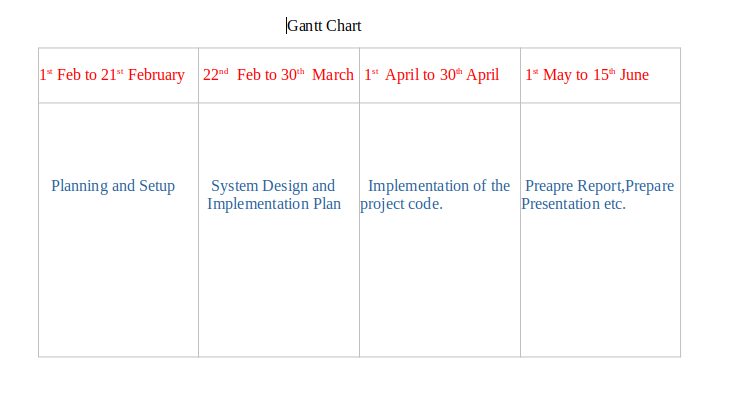
\includegraphics[width=0.95\linewidth]{images/ganttchart.png}
\caption{Gantt Chart}
\label{fig:1}
\end{figure}

\chapter{Related work}
\subsection*{Existing System Study}
The shortest path problem is about finding a path between  vertices in a graph such that the total sum of the edges weights is minimum.This problem can easily be solved with Dijkstra's Algorithm , Bellmon Ford Algorithm and Astar shortest path algorithm.But most of the shortest pathfinding tools uses the dijkstra's algorithm which is somewhat less efficient. \\
Various Algorithms such as such as Dijkstra's algorithm , Bellmon Ford Algorithm and Astar shortest path algorithm were studied and analysed for their space and time complexity.
\subsection*{Method of study}
The three important methods under qualitative analysis is used for studying existing system which are as follows:\\
(1)Observation: This includes observing different algorithms such as Dijkstra's algorithm , Bellmon Ford Algorithm and Astar shortest path algorithm in terms of their time and space compexity.\\
(2)In-depth research: This method includes going into the depth of algorithms , going through the proofs over which these algorithms relies.This method also goes into details how intuition for an algorithm was developed.\\
(3)Issues and questioning:This method helps to get information about the issues that have been faced or still facing with the existing systems. This can be used to modify the existing system as well as coming up with new solutions and exciting features.

\section{Comperative analysis}

Most of the shortest pathfinding tools uses the dijkstra's algorithm which is somewhat less efficient because in today world road connectivity is there between almost every two places which increases the number of both edges and vertices for the graph to represent an road network. So dijkstra's algorithm may work slower than expected in these kind of situations.To search for shortest path efficiently , shortest pathfinding tools should adopt much more efficient algorithms like Astar shortest path algorithm.

\section{Summary}
Shortest path algorithms have wide applications and so wide are no of algorithms to find shortest path.But the most important factor among all such algorithms are time and space complexity of the algorithms.We always want to use system which gives us faster results.Various Algorithms such as such as Dijkstra's algorithm , Bellmon Ford Algorithm and Astar shortest path algorithm were studied and analysed for their space and time complexity.In this project , I have analysed the Shortest path algorithms such as Dijkstra's algorithm and Astar search Algorithm etc. for time taken by the algorithms to find the shortest path . This Project also compares the shortest path algorithms over large dataset of nodes and edges for time taken by the algorithms. 






\chapter{System Design}

.....

\section{System design}
This project find the shortest path between cities of a state.Cities are taken as node and roads between them are taken as edges and the resultant graph is formed.The task is to find the shortest path between two cities (two nodes of the graph) of the california state efficiently.So, to complete the desired task the following system offers two algorithms namely dijkstra's algorithm for shortest path and Astar shortest path algorithm ..Both the algorihtms will work over large dataset of road network of california city.The dataset comprises 
almost 5 lac+ nodes and 20 lac+ edges.A shell program will also monitor the time taken by both algorithm to find shortest path between two nodes(cities) of the graph (Road network) . A graph is also plotted using gnuplot between time taken by both algrithms and no of nodes used.Gnuplot is used to plot graph between the time taken by an algorithm and no. of nodes used.
\subsection{Architecture}
This Project Architecture is usign Graph Data structures which is formed by reading large dataset of califorinia road network . The Dataset contains the Cities(nodes) and connections between nodes and distance between the nodes represented as Weight of the edges.
\newline
Dijkstra's algorithm for shortest path has been implemented in this project , Dijkstra's Algorithm is a greedy algorithm for solving single source shortest path problems that provides us with the shortest path from one particular given node to all other nodes in the graph.This algorithm finds the path with lowest cost(i.e. the shortest path) between that vertex and every other vertex.
\newline
A* algorithm is also used in this project .A* is a graph traversal and path search algorithm, which is considered to have ”brains” , it is known as intelligent algorithm as it chooses very optimal choice at every step.  The secret to its success is that it combines the pieces of information that Dijkstra’s Algorithm uses (favoring vertices that are close to the starting point) and information that Greedy Best-First-Search uses (favoring vertices that are close to the goal).  In the standard terminology used when talking about A*, g(n) represents the exact cost of the path from the starting point to any vertex n, and h(n)represents the heuristic estimated cost from vertex n to the goal.  Each time through the main loop, it examines the vertex n that has the lowest f(n) = g(n) + h(n).  What A* Search Algorithm does is that at each step it picks thenode according to a value-‘f’ which is a parameter equal to the sum of two other parameters – ‘g’ and ‘h’.  At eachstep it picks the node/cell having the lowest ‘f’, and process that node/cell.
\newline
This project also analyses the Dijkstra's Shortest path algorithm and Astar shortest path algorithm over a large dataset of road network of california state for time taken by both the algorithms to find the shortest path between two given cities(two nodes) of the graph.This file collects the time taken by both the algorithms and plot the graph between time taken and no. of nodes.


\newline
\newline




\chapter{Implementation}


....

\section{Experimental set-up description}

First for any algorithm to find shortest path , cost function f(n) is calculated.Then with help of following algorithm we calculates the shortest path .\\
\newline
\textbf{Algorithm :}\\
\newline
1) Create a Min Heap of size V where V is the number of vertices in the given graph. Every node of min heap contains vertex number and distance value of the vertex.\\
2) Initialize Min Heap with source vertex as root (the distance value assigned to source vertex is 0). The distance value assigned to all other vertices is INF (infinite).\\
3) While Min Heap is not empty, do following :\\
…..a) Extract the vertex with minimum distance value node from Min Heap. Let the extracted vertex be u.\\
…..b) For every adjacent vertex v of u, check if v is in Min Heap. If v is in Min Heap and distance value is more than weight of u-v plus distance value of u, then update the distance value of v.\\


Function f(n) is calculated as:\\

             f(n)=g(n)+h(n),\\
                   
For Disjkstra 's Algorithm : h(n)=0, So f(n)=g(n).\\
Control Flow Diagram of above algorithm is shown below:
\begin{figure}
\centering
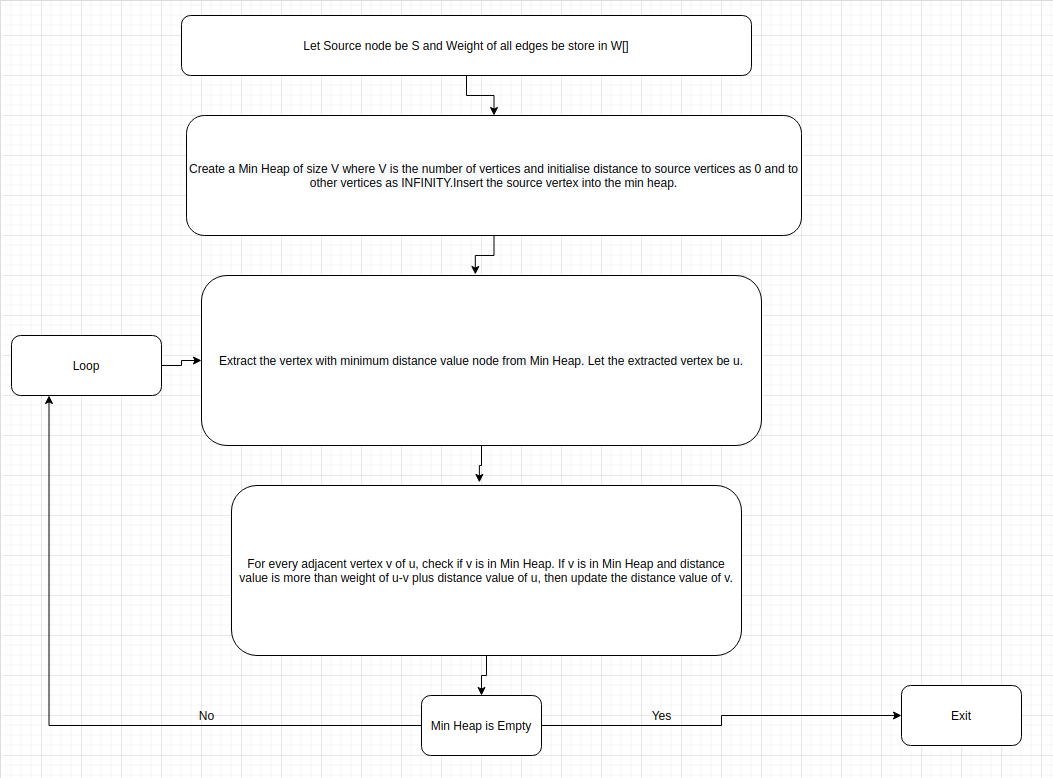
\includegraphics[width=1.1\linewidth,height=25cm]{control_flow}
\caption{Control Flow Diagram of the algorithm}
\label{fig:1}
\end{figure}

\newpage
\subsection{Function/Module/Class description}
This Section describes each modules of this project:\\
\newline
\textbf{1.dataset.txt:}
This file contains the huge road network of california.Dataset is having almost 5 lac+ nodes and 20 lac+ edges.
\\\\
\textbf{2.dijkstra.cpp:}
This module reads the dataset and forms the resultant graph from the dataset.Cities of the dataset are nodes of the graph and connection between the cities will be edges of the graph and distance between the cities will be weights of the edges of the graph.Dijkstra's algorithm for shortest path has been implemented in this module ,so lets understad dijkstra's algorithm:
Dijkstra's Algorithm is a greedy algorithm for solving single source shortest path problems that provides us with the shortest path from one particular given node to all other nodes in the graph.This algorithm finds the path with lowest cost(i.e. the shortest path) between that vertex and every other vertex .For example , if the vertices of the graph represent cities and edge path costs represent driving distances between pairs of cities connected by a direct road , Dijkstra's algorithm can be used to find the shortest route between one city and all other cities.
\\\\
\textbf{How it works?}\\
Let's create an array d[] where for each vertex v we store the current length of the shortest path from s to v in d[v]. Initially d[s]=0, and for all other vertices this length equals infinity. In the implementation a sufficiently large number (which is guaranteed to be greater than any possible path length) is chosen as infinity.\\
\\
           d[v]=INF, v!=s\\
\\
In addition, we maintain a Boolean array u[] which stores for each vertex v whether it's marked. Initially all vertices are unmarked:
\\\\
           u[v]=false\\
\\
The Dijkstra's algorithm runs for n iterations. At each iteration a vertex v is chosen as unmarked vertex which has the least value d[v]:\\

Evidently, in the first iteration the starting vertex s will be selected.\\

The selected vertex v is marked. Next, from vertex v relaxations are performed: all edges of the form (v,to) are considered, and for each vertex to the algorithm tries to improve the value d[to]. If the length of the current edge equals len, the code for relaxation is:
\\\\
           d[to]=min(d[to],d[v]+len)\\
           \\
After all such edges are considered, the current iteration ends. Finally, after n iterations, all vertices will be marked, and the algorithm terminates. We claim that the found values d[v] are the lengths of shortest paths from s to all vertices v.
\\\\
Note that if some vertices are unreachable from the starting vertex s, the values d[v] for them will remain infinite. Obviously, the last few iterations of the algorithm will choose those vertices, but no useful work will be done for them. Therefore, the algorithm can be stopped as soon as the selected vertex has infinite distance to it.
\\\\
\textbf{Algorithm:}\\
1) Create a Min Heap of size V where V is the number of vertices in the given graph. Every node of min heap contains vertex number and distance value of the vertex.\\
2) Initialize Min Heap with source vertex as root (the distance value assigned to source vertex is 0). The distance value assigned to all other vertices is INF (infinite).\\
3) While Min Heap is not empty, do following\\
…..a) Extract the vertex with minimum distance value node from Min Heap. Let the extracted vertex be u.\\
…..b) For every adjacent vertex v of u, check if v is in Min Heap. If v is in Min Heap and distance value is more than weight of u-v plus distance value of u, then update the distance value of v.\\
\\
Running Time complexity : O(E+V log V), where E-No. of edges in the graph , V-No. of vertices in the graph
\\\\
\textbf{3.Astar.hpp :} In this module the Astar search algorithm has been implemented for finding shortest path between two cities(two nodes of the graph).Astar search algorithm is implememted as a header file in C++ to provide cleaner code and code resuability(Concept of Polymorphism).Since This module implements the Astar search algorithm , so lets understand Astar search algorithm : 

A* is a graph traversal and path search algorithm, which is considered to have "brains" , it is known as intelligent algorithm as it chooses very optimal choice at every step.\\
The secret to its success is that it combines the pieces of information that Dijkstra’s Algorithm uses (favoring vertices that are close to the starting point) and information that Greedy Best-First-Search uses (favoring vertices that are close to the goal). In the standard terminology used when talking about A*, g(n) represents the exact cost of the path from the starting point to any vertex n, and h(n) represents the heuristic estimated cost from vertex n to the goal. Each time through the main loop, it examines the vertex n that has the lowest f(n) = g(n) + h(n).\\\\
What A* Search Algorithm does is that at each step it picks the node according to a value-‘f’ which is a parameter equal to the sum of two other parameters – ‘g’ and ‘h’. At each step it picks the node/cell having the lowest ‘f’, and process that node/cell.


g = the movement cost to move from one node to other node ,
h = the estimated movement cost to move from one node to other node. This is often referred to as the heuristic, which is nothing but a kind of smart guess. We really don’t know the actual distance until we find the path, because all sorts of things can be in the way (walls, water, etc.). There can be many ways to calculate this ‘h’ which are discussed as: 
\\\\
\textbf{Heuristics:}\\
We can calculate g but how to calculate h ?\\
\\
A* always requires a heuristic, it is defined using heuristic values for distances. A* in principle is just the ordinary Dijkstra algorithm using heuristic guesses for the distances.\\
\\
The heuristic function should run fast, in O(1) at query time. Otherwise we won't have much benefit from it. As heuristic we can select every function h for which:\\

1.h is admissible: h(u) \textless= dist(u, t) (never overestimate)\\
2.h is monotone: h(u) \textless= cost(u, v) + h(v) (triangle inequality)\\\\
There are however some heuristics that are frequently used in practice like:\\\\
\textbf{1.Straight-line heuristic:}\\
The straight-line distance (or as-the-crow-flies) is straightforward and easy to compute. For two nodes v, u we know the exact location, i.e. Longitude and Latitude.

We then just need to compute the straight-line distance by defining h as the Euclidean distance. 
This methods run in O(1).
\\\\
\textbf{2.Landmark heuristic:}\\
Here we need to pre-select some important nodes in our graph. Ideally we always choose a node that is part of frequently used shortest-paths.\\

However that knowledge is often not available so we can just select nodes that are farthest to the other selected landmarks. You can do so by using greedy farthest selection. Therefore we can do a Dijkstra from set which is very easy to implement. Just add multiple nodes at once into the Dijkstra starting queue (all current landmarks). Then run the Dijkstra until all distances have been computed and pick the node with greatest shortest-path distance as next landmark.
\\        \\    
\textbf{Algorithm:}\\
\\
1. make an openlist containing only the starting node\\
2. make an empty closed list\\
3.   while (the destination node has not been reached):\\
4. \hspace{10}       consider the node with the lowest f score in the open list\\
5.  \hspace{10}     if (this node is our destination node) :\\
6.   \hspace{20}        we are finished \\
7.  \hspace{10}     if not:\\
8.   \hspace{20}          put the current node in the closed list and look at all of its neighbors\\
9.    \hspace{20}         for (each neighbor of the current node):\\
10.   \hspace{20}              if (neighbor has lower g value than current and is in the closed list) :\\
11.     \hspace{40}               replace the neighbour with the new, lower, g value \\
12.      \hspace{40}              current node is now the neighbor's parent           \\ 
13.\hspace{20}                 else if (current g value is lower and this neighbour is in the open list ) :\\
14.  \hspace{40}                   replace the neighbour with the new, lower, g value \\
15.      \hspace{40}               change the neighbour's parent to our current node\\
16.  \hspace{20}          else if this neighbour is not in both lists:\\
17.    \hspace{40}                 add it to the open list and set its g\\
\\
Space Complexity : O(V) , V: no of vertices in the graph,\\
Time Complexity : O(E) , E: no of edges in the graph.
\\\\
Dijkstra's Algorithm is the special case of Astar shortest path algorithm  , In the cost function of Astar shortest path algorithm , i.e, f=g+h , where g=distance between the cities(edge weights) and h=heuristics cost .When h=0 , This becomes the dijkstra 's Algorithm.
\\

\textbf{4.Astar.cpp : }This module reads the dataset and forms the resultant graph from the dataset.Cities of the dataset are nodes of the graph and connection between the cities will be edges of the graph and distance between the cities will be weights of the edges of the graph. and apply the Astar search algorithm that is already implemented in Astar.hpp to find the shortest path between two cities(two nodes of the graph).
\\\\
\textbf{5.run.sh :} This module analyse the Dijkstra's Shortest path algorithm and Astar shortest path algorithm over a large dataset of road network of california state for time taken by both the algorithms to find the shortest path between two given cities(two nodes) of the graph.This file collects the time taken by both the algorithms and plot the graph between time taken and no. of nodes.
\\
\textbf{6.run.p :} This module plots the graph between the time taken by an algorithm and no. of nodes used.

\section{Obtained result}
The task is to find the shortest path between two cities (two nodes of the graph) of the california state efficiently.So, to complete the desired task the following system offers two algorithms namely dijkstra's algorithm for shortest path and Astar shortest path algorithm .Lets see result of both algorithms one by one.\newline
\\
\textbf{1.Dijkstra.cpp:}\newline
This file reads the dataset of nodes and edges and form the corresponding graph.This file also takes the destination city (destination node) to which path is to be found.And then this file displays the time taken by the algorithm to find the path and distance of the resultant shortest path.
\newline
\\
\textbf{2.Astar.cpp:}\newline
This file reads the dataset of nodes and edges and form the corresponding graph.This file also takes the destination city (destination node) to which path is to be found.And then this file displays the time taken by the algorithm to find the path and distance of the resultant shortest path.Astar algorithm doesn't always guarantees the shortest path as it depends on the heuristic function taken.
\newline
\\
\textbf{3.run.sh:}\newline
This file analyse the Dijkstra's Shortest path algorithm and Astar shortest path algorithm over a large dataset of road network of california state for time taken by both the algorithms to find the shortest path between two given cities(two nodes) of the graph.This file collects the time taken by both the algorithms and plot the graph between time taken and no. of nodes.
\\\\\\\\\\\\
So,the result obtained is the time taken to find the shortest path and length of the shortest path between two given cities(two nodes of the graph) of the california road network namely source city and destination city provided to the Dijkstra's program and Astar's Program as command line input .
The shell program also plot the graph between the time taken and no. of nodes used by both Dijkstra's Algorithm and Astar Algorithm.The project output also compares between the time taken by both the algorithm to find their shortest path .
\chapter{Result analysis and Testing}

\section{Testing}
The Project programs are  tested over the large dataset of graph network.The dataset represents the california state road network between the cities.The dataset contains almost 5 lac+ nodes and 20 lac+ edges ,which makes the resultant graph much more dense.But it is interesting to note the observations for such denser graphs.Image of the Dataset is represented by fig.5.1 .First  Column represents the source node(Source City) , Second column represents the destination node(Destination City) and third column represents the weights of the edges(Distance between the city).
\begin{figure}
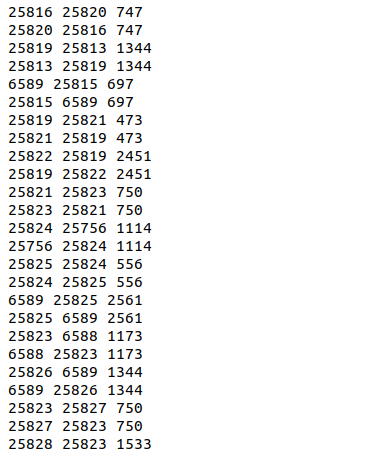
\includegraphics[]{images/dataset.png}
\caption{Image of the Dataset}
\label{fig:1}
\end{figure}
\section{Result Analysis}
\textbf{1.dijkstra.cpp :}\newline
This file takes destination city (Destination node) as command line input and displays the shortest path length and time taken by the algorithm to find the shortest path.The sample output of this file is represented by fig 5.2.
\begin{figure}
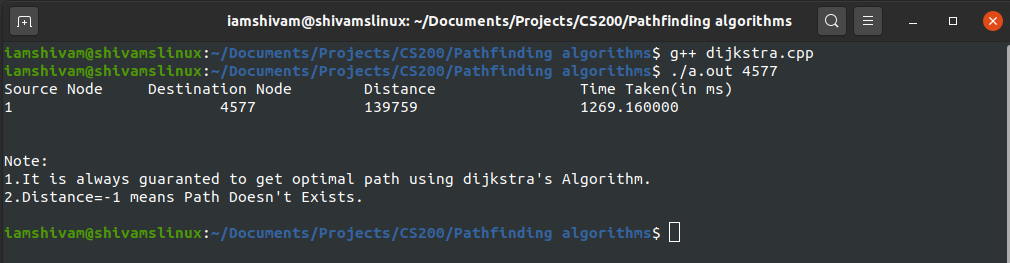
\includegraphics[width=24cm]{images/dijkstra.png}
\caption{Output of the dijkstra's Algorithm}
\label{fig:1}
\end{figure}
\newline
\\
\textbf{2.astar.cpp :}\newline
This file takes destination city (Destination node) as command line input and displays the shortest path length and time taken by the algorithm to find the shortest path.The sample output of this file is represented by fig 5.3.
\newline
\begin{figure}
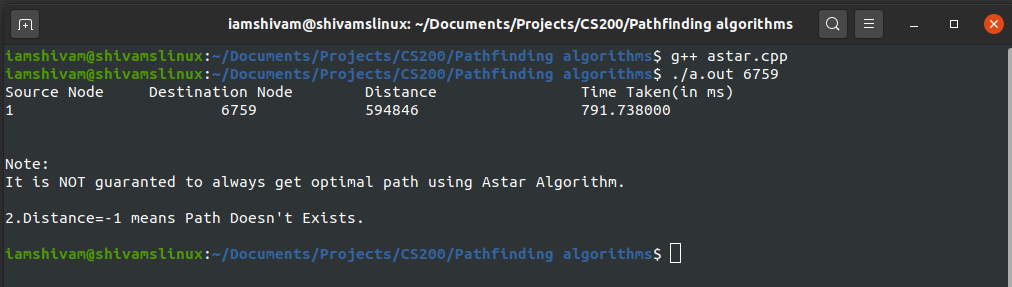
\includegraphics[width=24cm]{images/astar.png}
\caption{Output of the  Astar Algorithm}
\label{fig:1}
\end{figure}
\\
\textbf{3.run.sh :}\newline
This file takes destination city (Destination node) as command line input and displays the shortest path length and time taken by the algorithm to find the shortest path.The sample output of this file is represented by fig 5.4.
\newline
\begin{figure}
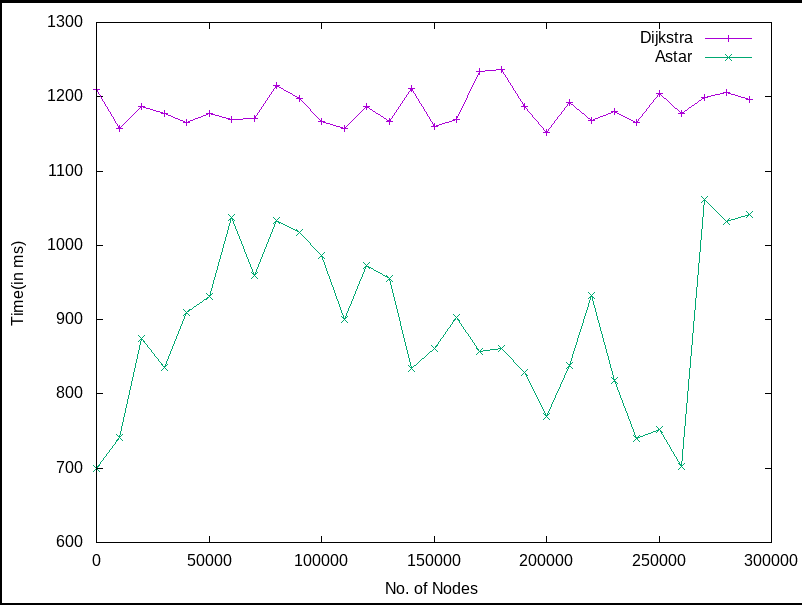
\includegraphics[width=18cm]{images/compare.png}
\caption{Comparison between Dijkstra's and Astar algorithm}
\label{fig:1}
\end{figure}
\chapter{Conclusion and Future work }

\section{Conclusion}
Shortest path algorithms have many applications.Mapping software like Google or Apple maps makes use of shortest path algorithms.Shortest path algorithms have wide applications and so wide are no of algorithms to find shortest path.But the most important factor among all such algorithms are time and space complexity of the algorithms.We always want to use system which gives us faster results.In this project , we have analysed the Shortest path algorithms such as Dijkstra's algorithm and Astar search Algorithm etc. for time taken by the algorithms to find the shortest path . This Project also compares the shortest path algorithms over large dataset of nodes and edges for time taken by the algorithms. 
\section{Future Work}
This Project was all about analysing single source shortest path . In future , this project can be extended to analyse All pairs Shortest path algorithms and compare between them for time complexity over large dataset.The goal of the all-pair-shortest-paths problem is to find the shortest path between all pairs of nodes of the graph. 
\section* {Bibliography}
[1] T.H.Cormen,C.E.Leiserson,R.L.Rivest and C Stein, \textit{\enquote{Introduction to Algorithms. }}\\ \relax
[2] http://theory.stanford.edu/~amitp/GameProgramming/AStarComparison.html, \textit{\enquote{Introduction to A*}},\\ \relax

\bibliographystyle{ieeetr}
\bibliography{project} 
\end{document}

